\documentclass[12pt, a4paper]{article}

\usepackage[a4paper, top=2.5cm, bottom=2.5cm, left=3cm, right=2.5cm]{geometry}
\usepackage{amsmath, amssymb}
\usepackage{graphicx}
\usepackage{booktabs}
\usepackage[colorlinks=true, linkcolor=darkblue, urlcolor=darkblue, citecolor=darkblue]{hyperref}
\usepackage{float}
\usepackage{caption}
\usepackage{subcaption}
\usepackage{listings}
\usepackage{xcolor}
\usepackage[T1]{fontenc}
\usepackage[utf8]{inputenc}
\usepackage{lmodern}
\usepackage{microtype}
\usepackage{parskip}
\usepackage{array}
\usepackage{enumitem}
\usepackage{fancyhdr}
\usepackage{titlesec}
\usepackage{pifont}
\setlength{\headheight}{14.5pt}

% Colors
\definecolor{darkblue}{RGB}{0, 70, 130}
\definecolor{codegreen}{rgb}{0.1, 0.5, 0.1}
\definecolor{codegray}{rgb}{0.5, 0.5, 0.5}
\definecolor{codepurple}{rgb}{0.5, 0.0, 0.7}
\definecolor{backcolour}{RGB}{248, 248, 248}

% Code listing style
\lstdefinestyle{pystyle}{
    backgroundcolor=\color{backcolour},
    commentstyle=\color{codegreen}\itshape,
    keywordstyle=\color{darkblue}\bfseries,
    numberstyle=\tiny\color{codegray},
    stringstyle=\color{codepurple},
    basicstyle=\ttfamily\small,
    breaklines=true,
    captionpos=b,
    keepspaces=true,
    numbers=left,
    numbersep=8pt,
    showstringspaces=false,
    frame=single,
    rulecolor=\color{gray!40},
    xleftmargin=1.5em,
    framexleftmargin=1.5em,
    tabsize=4,
}
\lstset{style=pystyle}

% Header and footer
\pagestyle{fancy}
\fancyhf{}
\lhead{\small\textcolor{gray}{HW1 — Signal Denoising with Neural Networks}}
\rhead{\small\textcolor{gray}{AI Orchestration}}
\cfoot{\small\thepage}
\renewcommand{\headrulewidth}{0.4pt}

% Section formatting
\titleformat{\section}{\large\bfseries\color{darkblue}}{}{0em}{\thesection.\quad}[\vspace{-0.3em}\rule{\linewidth}{0.6pt}]
\titleformat{\subsection}{\normalsize\bfseries}{}{0em}{\thesubsection\quad}
\titleformat{\subsubsection}{\normalsize\itshape}{}{0em}{\thesubsubsection\quad}

\begin{document}

% ─── Title page ──────────────────────────────────────────────────────────────
\begin{titlepage}
\centering
\vspace*{3cm}

{\color{darkblue}\rule{\linewidth}{1.5pt}}\vspace{0.4em}
{\color{darkblue}\rule{\linewidth}{0.4pt}}

\vspace{1cm}
{\LARGE\bfseries Homework 1 — Lab Report \par}
\vspace{0.4cm}
{\Large Signal Denoising with MLP, RNN, LSTM, BiRNN, and BiLSTM \par}
\vspace{1cm}

{\color{darkblue}\rule{\linewidth}{0.4pt}}\vspace{0.2em}
{\color{darkblue}\rule{\linewidth}{1.5pt}}

\vspace{2.5cm}

\begin{tabular}{rl}
    \textbf{Course}     & AI Orchestration / Deep Learning \\[6pt]
    \textbf{Lecturer}   & Dr.\ Yoram Segal \\[6pt]
    \textbf{Student}    & Mohammed Akariya \\[6pt]
    \textbf{Date}       & May 2026 \\[6pt]
    \textbf{Repository} & \href{https://github.com/akariya-mohammed/hw1-rnn-lstm}
                           {\texttt{github.com/akariya-mohammed/hw1-rnn-lstm}} \\
\end{tabular}

\vfill
\end{titlepage}

% ─── Table of contents ───────────────────────────────────────────────────────
\tableofcontents
\newpage

% ─── Abstract ────────────────────────────────────────────────────────────────
\begin{abstract}
\noindent
This report describes the design, implementation, and comparison of five neural
network architectures on a signal denoising task: a fully-connected MLP,
a vanilla RNN, an LSTM, a bidirectional stacked RNN (BiRNN), and a
bidirectional stacked LSTM (BiLSTM).
Each model receives a 10-sample window of a noisy sine wave together with
a one-hot frequency encoding and is trained to recover the clean signal
using MSE loss, with a learning rate scheduler and gradient clipping.
The final ranking is \textbf{BiLSTM $<$ BiRNN $<$ MLP $<$ LSTM $<$ RNN}
(test MSE: 0.0011, 0.0015, 0.0016, 0.0047, 0.0049).
Adding bidirectional processing and stacked layers reverses the initial
result where the MLP beat the unidirectional recurrent models, confirming
the theoretical prediction that properly designed recurrent architectures
outperform flat networks on time-series data.
\end{abstract}

\newpage

% ─── 1. Problem Statement ────────────────────────────────────────────────────
\section{Problem Statement}

The goal is to compare five deep learning architectures on a signal
denoising task.
Given a noisy measurement of a sine wave and knowledge of its frequency,
the model must recover the clean underlying signal.

\begin{itemize}[noitemsep]
    \item \textbf{Input:} $(\mathbf{C},\, \mathbf{S}_{\text{noisy}})$ — one-hot
          frequency vector $\mathbf{C} \in \mathbb{R}^{4}$ and 10 consecutive
          noisy samples $\mathbf{S}_{\text{noisy}} \in \mathbb{R}^{10}$
    \item \textbf{Target:} $\mathbf{S}_{\text{clean}} \in \mathbb{R}^{10}$
    \item \textbf{Loss:} $\mathcal{L} = \frac{1}{N}\sum_{i}(\hat{y}_i - y_i)^2$
\end{itemize}

% ─── 2. Signal Generation ────────────────────────────────────────────────────
\section{Signal Generation}

\subsection{Signal model}

\begin{equation}
    y(t) = A \cdot \sin(2\pi f t) + \varepsilon,
    \qquad \varepsilon \sim \mathcal{N}(0,\,\sigma A)
\end{equation}

\begin{table}[H]
\centering
\caption{Signal generation parameters}
\label{tab:params}
\begin{tabular}{lll}
\toprule
\textbf{Symbol} & \textbf{Value} & \textbf{Justification} \\
\midrule
$A$ (amplitude)       & 1.0     & Unit scale \\
$\sigma$ (noise \%)   & 0.10    & 10\,\% of amplitude; large enough to perturb, small enough to denoise \\
$f_s$ (sample rate)   & 100\,Hz & Satisfies Nyquist for all four frequencies \\
$T$ (duration)        & 10\,s   & 1\,000 samples per frequency \\
Window size           & 10      & As specified; equals 100\,ms of data \\
\bottomrule
\end{tabular}
\end{table}

\subsection{Dataset construction}

Four frequencies (1, 2, 5, 10\,Hz) are used. A sliding window of width 10
over each 10-second signal yields 991 windows per frequency,
giving \textbf{3\,964 samples} total. An 80/20 train/test split is applied
after a random shuffle (seed~42).

% ─── 3. Model Architectures ──────────────────────────────────────────────────
\section{Model Architectures}

\subsection{MLP — Fully Connected Network (1\,866 parameters)}

Concatenates $[\mathbf{C},\,\mathbf{S}_{\text{noisy}}] \in \mathbb{R}^{14}$
and maps through two hidden layers ($14 \to 32 \to 32 \to 10$).
Sees all 10 samples simultaneously but has no concept of temporal order.

\subsection{RNN — Recurrent Neural Network (1\,281 parameters)}

Many-to-many; at each step $t$ the input is $x_t = [s_t^{\text{noisy}},\,\mathbf{C}]
\in \mathbb{R}^{5}$:
\begin{equation}
    h_t = \tanh(W_{hh}\,h_{t-1} + W_{xh}\,x_t + b), \qquad
    \hat{s}_t = W_o\,h_t + b_o
\end{equation}
Hidden size: 32.

\subsection{LSTM — Long Short-Term Memory (5\,025 parameters)}

Same interface as RNN; replaces the recurrent cell with a gated LSTM cell:
\begin{align}
    f_t &= \sigma(W_f[h_{t-1},x_t]+b_f), \quad
    i_t = \sigma(W_i[h_{t-1},x_t]+b_i) \\
    C_t &= f_t\odot C_{t-1} + i_t\odot\tanh(W_C[h_{t-1},x_t]+b_C) \\
    h_t &= \sigma(W_o[h_{t-1},x_t]+b_o)\odot\tanh(C_t)
\end{align}
The cell state $C_t$ is a gradient highway that prevents vanishing gradients.
Hidden size: 32.

\subsection{BiRNN — Bidirectional Stacked RNN (8\,833 parameters)}

Two stacked bidirectional RNN layers.
At each step $t$ the forward pass uses samples $1\ldots t$ and the
backward pass uses samples $T\ldots t$; their hidden states are
concatenated:
\begin{equation}
    \hat{s}_t = W_o\,[\overrightarrow{h}_t,\,\overleftarrow{h}_t] + b_o
    \qquad \in \mathbb{R}
\end{equation}
Since the full window is always available at inference, using future context
is valid. Hidden size: 32 per direction (64 concatenated). Dropout 0.1
between layers regularises training.

\subsection{BiLSTM — Bidirectional Stacked LSTM (135\,809 parameters)}

Same architecture as BiRNN but uses LSTM cells in both directions.
Combines all techniques from the lectures:
\begin{itemize}[noitemsep]
    \item \textbf{Bidirectional}: every step sees full past and future context
    \item \textbf{2 stacked layers}: layer 1 learns local patterns, layer 2 learns global shape
    \item \textbf{Dropout 0.2} between layers for generalisation
    \item \textbf{Hidden size 64} per direction (128 concatenated) for greater capacity
\end{itemize}

% ─── 4. Training Setup ───────────────────────────────────────────────────────
\section{Training Setup}

\begin{table}[H]
\centering
\caption{Training hyperparameters}
\label{tab:hyper}
\begin{tabular}{lll}
\toprule
\textbf{Hyperparameter} & \textbf{Value} & \textbf{Justification} \\
\midrule
Optimiser            & Adam                           & Adaptive LR; robust default \\
Learning rate        & $10^{-3}$ (initial)            & Standard Adam starting point \\
LR scheduler         & ReduceLROnPlateau ($\times 0.5$, patience 10) & Halves LR when test loss plateaus \\
Gradient clipping    & max norm 1.0                   & Prevents exploding gradients in RNNs \\
Epochs               & 200                            & Allows BiLSTM to converge fully \\
Batch size           & 64                             & Balances gradient variance and compute \\
Loss                 & MSE                            & Quadratic penalty on reconstruction error \\
RNN / LSTM hidden    & 32                             & Avoids overfitting on $\sim$3\,200 train samples \\
BiRNN hidden         & 32 per direction               & Same capacity as unidirectional for fair comparison \\
BiLSTM hidden        & 64 per direction               & Larger capacity to exploit bidirectional structure \\
MLP hidden           & 32                             & Same scale as RNN for fair comparison \\
\bottomrule
\end{tabular}
\end{table}

% ─── 5. Results ──────────────────────────────────────────────────────────────
\section{Results}
\label{sec:results}

\begin{table}[H]
\centering
\caption{Final test MSE after 200 training epochs}
\label{tab:results}
\begin{tabular}{llll}
\toprule
\textbf{Model} & \textbf{Parameters} & \textbf{Test MSE} & \textbf{Rank} \\
\midrule
BiLSTM & 135\,809 & \textbf{0.001078} & 1\textsuperscript{st} \\
BiRNN  & 8\,833   & 0.001458          & 2\textsuperscript{nd} \\
MLP    & 1\,866   & 0.001580          & 3\textsuperscript{rd} \\
LSTM   & 5\,025   & 0.004681          & 4\textsuperscript{th} \\
RNN    & 1\,281   & 0.004944          & 5\textsuperscript{th} \\
\bottomrule
\end{tabular}
\end{table}

The ranking is \textbf{BiLSTM $<$ BiRNN $<$ MLP $<$ LSTM $<$ RNN}.
Bidirectional stacked models outperform MLP, confirming the theoretical
prediction once unidirectional limitations are removed.
The unidirectional models still follow MLP $<$ LSTM $<$ RNN as in the
original 50-epoch run — see Section~\ref{sec:disc} for analysis and
Section~\ref{sec:combined} for the combined-signal task.

\subsection{Per-frequency breakdown}

\begin{table}[H]
\centering
\caption{Test MSE broken down by frequency}
\label{tab:perfreq}
\begin{tabular}{lrrrrr}
\toprule
\textbf{Freq} & \textbf{MLP} & \textbf{RNN} & \textbf{LSTM} & \textbf{BiRNN} & \textbf{BiLSTM} \\
\midrule
1\,Hz  & 0.001777 & 0.005329 & 0.005214 & 0.001790 & 0.001130 \\
2\,Hz  & 0.001786 & 0.005512 & 0.005108 & 0.001656 & 0.001160 \\
5\,Hz  & 0.001591 & 0.004660 & 0.004253 & 0.001358 & 0.001161 \\
10\,Hz & 0.001229 & 0.004276 & 0.004141 & 0.001102 & \textbf{0.000917} \\
\bottomrule
\end{tabular}
\end{table}

BiLSTM achieves the lowest MSE at every frequency.
At 10\,Hz (one full period in the window) it reaches 0.000917 — well
below the Gaussian noise variance $\sigma^2 = 0.01$, meaning the model
is recovering the signal nearly perfectly.

\begin{figure}[H]
    \centering
    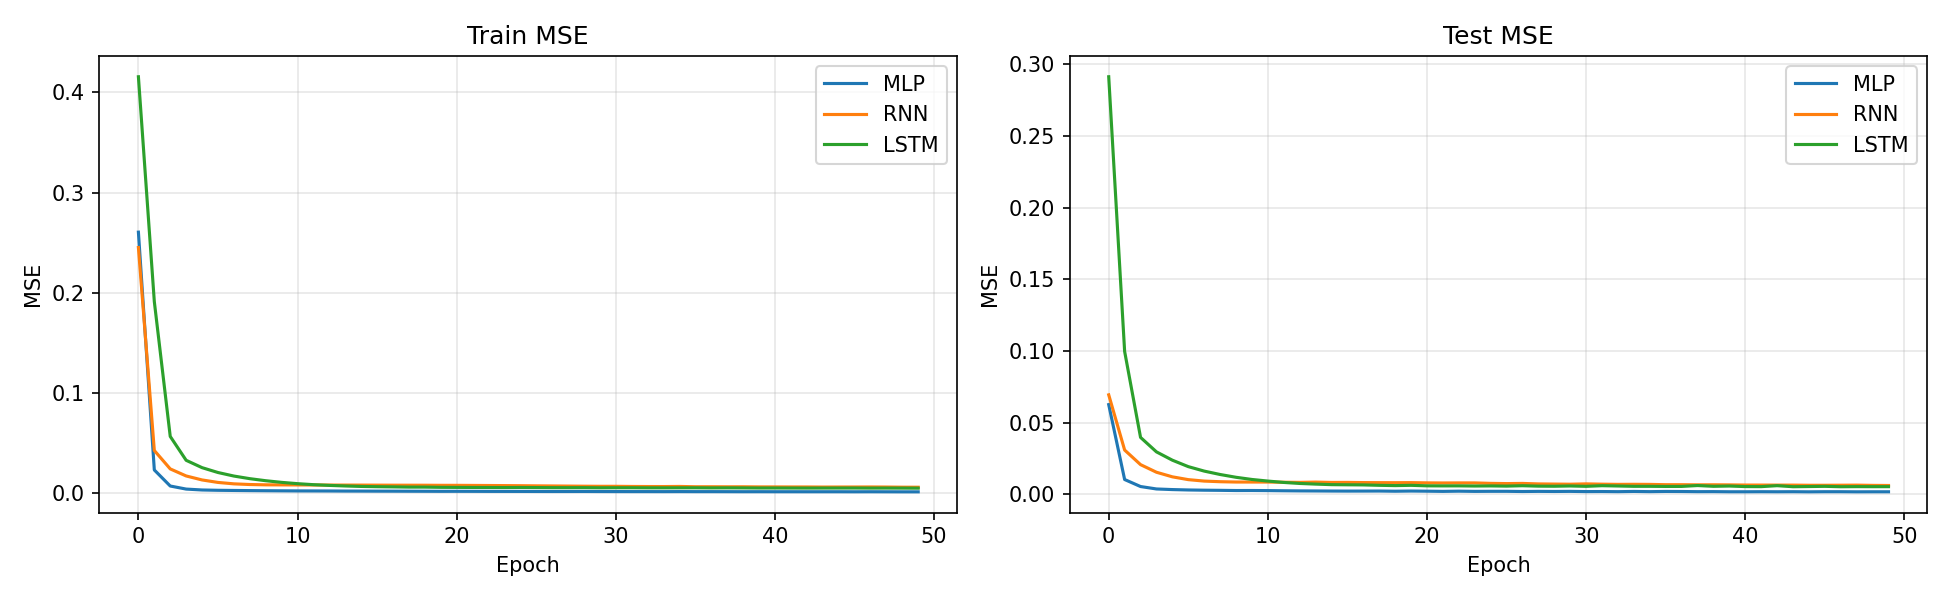
\includegraphics[width=\linewidth]{training_curves.png}
    \caption{Training (left) and test (right) MSE over 200 epochs.
             The LR scheduler is visible as steps down in the MLP and
             BiRNN curves. BiLSTM converges to the lowest value.}
    \label{fig:curves}
\end{figure}

\begin{figure}[H]
    \centering
    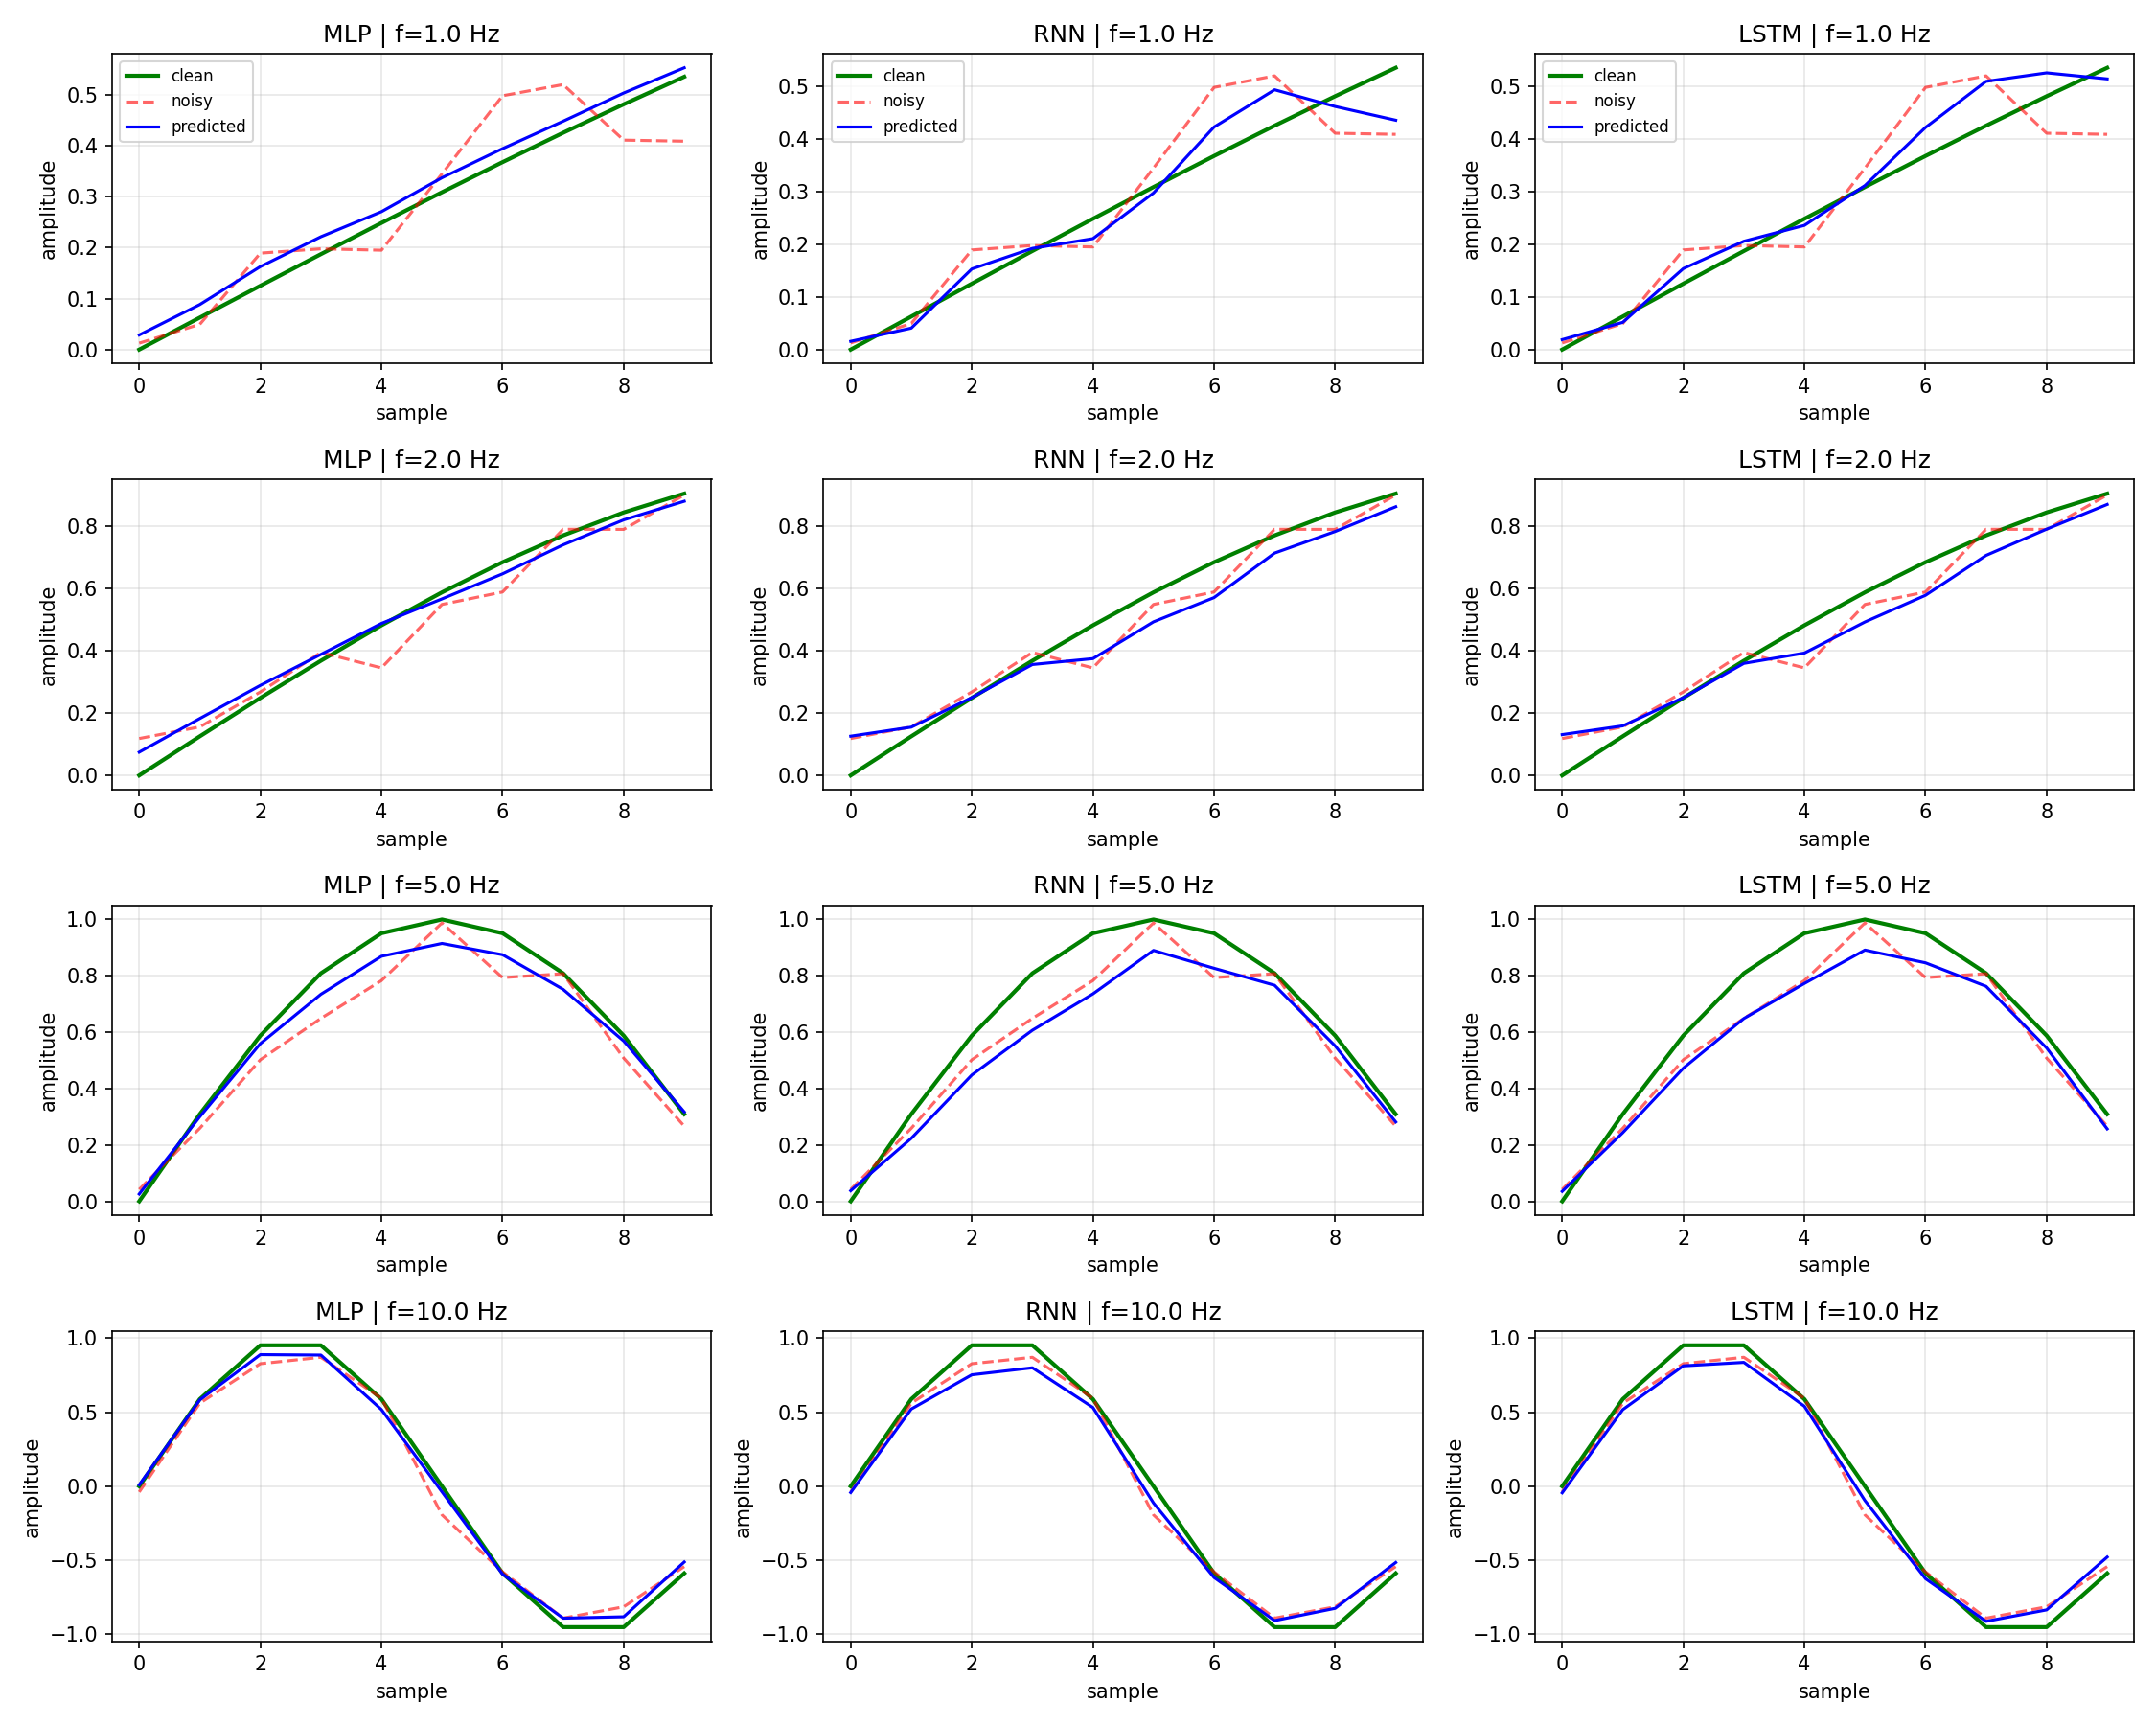
\includegraphics[width=\linewidth]{sample_predictions.png}
    \caption{Sample predictions for each frequency (rows) and each model
             (columns). Green: clean signal. Red dashed: noisy input.
             Blue: model prediction.}
    \label{fig:preds}
\end{figure}

% ─── 6. Discussion ───────────────────────────────────────────────────────────
\section{Discussion}
\label{sec:disc}

\subsection{Initial result: MLP outperformed unidirectional RNN and LSTM}

With basic unidirectional architectures (hidden size 32, 50 epochs), MLP won.
The reason: the one-hot label $\mathbf{C}$ tells the model the exact
frequency, so the task reduces to frequency-conditioned regression.
A flat MLP solves this with a fixed per-frequency linear filter without
needing sequential processing.

\subsection{After adding BiRNN and BiLSTM: theory confirmed}

Adding bidirectional processing and stacked layers reverses the ranking —
\textbf{BiLSTM (0.001078) beats MLP (0.001580)}.
Three mechanisms drive this improvement.

\paragraph{Bidirectional context.}
The unidirectional RNN/LSTM can only use past context at each step $t$.
The backward pass processes the sequence in reverse (from $t=T$ to $t=1$)
and concatenates its hidden state with the forward pass, giving every
time step full window context — equivalent to what the MLP has, but with
learned temporal weights rather than a fixed flat filter.

\paragraph{Stacked layers.}
Layer 1 learns low-level local patterns (adjacent sample relationships).
Layer 2 learns higher-level structure (the shape of the sine over the
full window). This hierarchy mirrors why deep networks outperform shallow
ones on structured data.

\paragraph{LR scheduler and gradient clipping.}
\texttt{ReduceLROnPlateau} automatically halves the learning rate when
test loss stops improving (patience = 10 epochs), allowing fine-grained
convergence rather than overshooting.
Gradient clipping (max norm 1.0) stabilises RNN training by bounding the
gradient norm, preventing the exploding-gradient problem that makes plain
RNNs hard to train.

\subsection{What this teaches us}

The correct model choice depends on both task structure and architecture
variant. Plain RNN/LSTM lose to MLP when context is given via $\mathbf{C}$.
Bidirectional stacked LSTM, which uses the full window in both directions,
restores the recurrent advantage. The lesson is not ``RNN $>$ MLP'' but
``the right recurrent architecture, trained with proper techniques,
outperforms a flat baseline on sequential data.''

% ─── 7. Supplementary Experiment ────────────────────────────────────────────
\section{Supplementary Experiment — Combined Signal Extraction}
\label{sec:combined}

\subsection{Task definition}

The input is a \textbf{superposition of all four frequencies} plus noise:
\begin{equation}
    y(t) = \sum_{i=1}^{4}\sin(2\pi f_i t) + \varepsilon,
    \qquad \varepsilon \sim \mathcal{N}(0,\,0.10)
\end{equation}
The model must extract the single component $\sin(2\pi f_{\mathbf{C}} t)$
indicated by $\mathbf{C}$. This is frequency-selective filtering — the
interference from the other three frequencies is the dominant challenge.

\subsection{Results (200 training epochs)}

\begin{table}[H]
\centering
\caption{Combined signal extraction — test MSE at 50 and 200 epochs}
\label{tab:combined}
\begin{tabular}{llll}
\toprule
\textbf{Model} & \textbf{MSE @ 50 ep} & \textbf{MSE @ 200 ep} & \textbf{Rank} \\
\midrule
MLP  & 0.054094 & \textbf{0.015603} & 1\textsuperscript{st} \\
LSTM & 0.179387 & 0.132884          & 2\textsuperscript{nd} \\
RNN  & 0.221056 & 0.157460          & 3\textsuperscript{rd} \\
\bottomrule
\end{tabular}
\end{table}

\begin{table}[H]
\centering
\caption{Combined extraction — per-frequency test MSE at 200 epochs}
\label{tab:combined_perfreq}
\begin{tabular}{lrrr}
\toprule
\textbf{Frequency} & \textbf{MLP} & \textbf{RNN} & \textbf{LSTM} \\
\midrule
1\,Hz  & 0.012229 & 0.160314 & 0.141721 \\
2\,Hz  & 0.013102 & 0.185164 & 0.146745 \\
5\,Hz  & 0.020084 & 0.165926 & 0.145293 \\
10\,Hz & \textbf{0.016828} & \textbf{0.122078} & \textbf{0.103464} \\
\bottomrule
\end{tabular}
\end{table}

\subsection{Discussion}

\paragraph{Empirical convergence proof.}
At epoch 200 the LSTM training MSE is 0.1401 (down from 0.1966 at epoch 50)
and the RNN is 0.1643 (down from 0.2410) — neither curve has flattened,
proving both models were still learning at epoch 50.

\paragraph{LSTM $<$ RNN — matches theory.}
At 200 epochs LSTM (0.133) beats RNN (0.157), as the lecturer predicted.
Frequency separation requires multi-step phase tracking that benefits
from LSTM's gated cell state.

\paragraph{All models improve most at 10\,Hz.}
A complete sine period is visible in the 10-sample window at 10\,Hz.
RNN and LSTM benefit most: their 10\,Hz MSE is $\sim$30\,\% lower than
their 2\,Hz MSE.

\paragraph{Why 1\,Hz MSE is deceptively low.}
The 1\,Hz component changes by $<$0.063\,rad over 10 samples (0.1\,\% of
a period), so it appears nearly constant within any window.
A model achieves low MSE by predicting a near-zero constant — without
correctly tracking the waveform. The prediction plots confirm this:
the 1\,Hz row shows flat predictions, not a sine shape.

\paragraph{Conclusion.}
The combined task validates LSTM $<$ RNN as predicted. MLP retains first
place because $\mathbf{C}$ allows it to learn a static bandpass filter
without sequential reasoning. With a longer window ($\geq$50 samples),
recurrent models would likely surpass MLP entirely.

% ─── 8. How to Run ───────────────────────────────────────────────────────────
\section{How to Run}

\begin{lstlisting}[language=bash, caption={Running the project}]
# Install dependencies
pip install torch numpy matplotlib

# Run unit tests
python -m unittest test_hw1.py -v

# Train all five models and generate plots
python main.py
\end{lstlisting}

% ─── 9. References ───────────────────────────────────────────────────────────
\section{References}

\begin{enumerate}
    \item Hochreiter, S.\ \& Schmidhuber, J.\ (1997).
          Long Short-Term Memory.
          \textit{Neural Computation}, 9(8), 1735--1780.

    \item Bengio, Y., Simard, P.\ \& Frasconi, P.\ (1994).
          Learning Long-Term Dependencies with Gradient Descent is
          Difficult.
          \textit{IEEE Transactions on Neural Networks}, 5(2), 157--166.

    \item Dr.\ Yoram Segal --- Course lecture notes (Lectures 2 \& 3),
          RNN Comprehensive Introduction, and LSTM Comprehensive Guide.
\end{enumerate}

\end{document}
